\chapter{Comunicazione}

In questo capitolo sarà proposto una modellizzazione della trasmissione di informazione attraverso canali comunicanti. 

\section{Trasmissione di informazione}
\label{sec:Trasmissione}

Il modello più semplice sarà costituito da una sorgente, un canale di comunicazione, ed un ricevente.\\
La sorgente sarà modellata da una variabile aleatoria $S$ con valori \va detti alfabeto sorgente e \lep. Il fatto che la sorgente $S$ sia una variabile casuale va interpretata come l'incertezza su quale sarà il messaggio inviato. in questo contesto un messaggio sarà una serie di simboli da \va uno di seguito all'altro.
il ricevente sarà un'altra variabile casuale $R$ con valori \vb  detti alfabeto ricevente e \leggeq. Solitamente avremo che $m \geq n$. Infine l'effetto di distorsione del canale sarà modellato dalla famiglia di probabilità condizionate \lepc  dove $p(j|i):= \mathbb{P}(R=b_j|S=a_i)$ (corrisponde a $p_i(j)$ definito in \ref{sec:PropriEntropia}). Un sistema di trasmissione ottimale avrà i due alfabeti di trasmissione e ricezione identici e nella distorsione avremo $p(i|i)$ il più vicino possibile ad 1.\\
\begin{defi}
viene detta \textbf{mutua informazione}  tra due eventi $E(S=a_j)$ ed $F(R=b_k)$ il valore:
\begin{equation}
I(a_j,b_k)=-log(q_k)+ log(p(k|j))
\end{equation}
se $p_j=0$ allora diremo $I(a_j,b_k)=0$.
\end{defi}
È importante notare che questa definizione di mutua informazione è diversa da \ref{defi:mutua}  data che si riferisce a due variabili casuali.\\
Dato che $-log(q_k)$ è l'informazione dell'evento $R=b_k$, mentre $-log(p(k|j))$ è l'informazione aggiuntiva che ci darebbe la ricezione di $b_k$ sapendo già per certo che è stato spedito $a_j$, possiamo interpretare $I(a_j,b_k)$ come la quantità di informazione su $R=b_k$ che ci è data dall'evento $S=a_j$. In altre parole è la quantità di informazione che è spedita attraverso il canale. Notiamo che se non ci fosse rumore ($p(i|i)=1$) avremmo che:
$$I(a_j,b_k)=-log(q_k)=I(q_k)$$
\begin{teo}
Per ogni $1\leq j \leq n , 1 \leq k, \leq m$ si ha:
\begin{enumerate}
\item $I(a_j,b_k)=-log(\frac{p_jk}{p_j q_k})$
\item $I(a_j,b_k)=-log(p_j)+log(q(j|k))$
\item $I(a_j,b_k)=I(b_k,a_j)$
\item se gli eventi $S=a_j$ e $R=b_k$ sono indipendenti allora $I(a_j,b_k)=0$
\item $I(S,R)=\sumj \sumk p_{jk}I(a_j,b_k)$.
\end{enumerate}
\end{teo}
\begin{proof}
\begin{enumerate}
\item deriva banalmente da $p(k|j)=\frac{p_{jk}}{q_k}$
\item si ricava sostituendo in 1. $q(j|k)=\frac{p_{ik}}{q_k}$
\item deriva da 2.
\item ricordando che nel caso siano indipendenti $p_{jk}=p_jq_k$ si ricava immediatamente da da 1.
\item si ricava da 1. e dal primo punto del teorema \ref{teo:6.7}
\end{enumerate}
\end{proof}

Il punto 3. del sistema ci mostra la curiosa caratteristica per cui se in un sistema si invertono sorgente e ricevente abbiamo che l'informazione su $a_j$ contenuta in $b_k$ è la stessa di quella contenuta in $a_j$ su $b_k$ quando il canale funziona normalmente. Il punto 5. invece esprime la mutua informazione tra due variabili casuali definita in \ref{defi:mutua} come la media di tutte le possibili trasmissioni dei singoli simboli. Si può dimostrare che $I(S,R)\geq 0$ sempre.\\

Supponiamo ora preso un canale, di fissare \lepc . Vogliamo ora fare in modo che il canale trasmetta più informazione possibile, per fare ciò le uniche variabili del sistema rimaste ancora libere sono $\{p_1...p_n \}$ .
\begin{defi}
viene definita \textbf{capacità del canale C} la quantità:
\begin{equation}
C:=max I(S,R)
\end{equation}
dove il massimo è scelto tra tutte le possibili leggi di probabilità della variabile $S$
\end{defi}
Operativamente spesso è preferibile vedere la capacità del canale C come:
\begin{equation}
C=max(H(R)-H_s(R))
\end{equation}
ottenuta utilizzando la definizione \ref{defi:mutua}.\\
\begin{oss} \label{oss:bsc}
Il più semplice esempio di canale di comunicazione che possiamo trovare è un canale binario simmetrico, esso avrà grande rilevanza in seguito.\\
È formato da una sorgente  con alfabeto $\{ 0 , 1 \}$ e come specificato nella figura il \textit{rumore} del canale è definito attraverso un parametro $p$


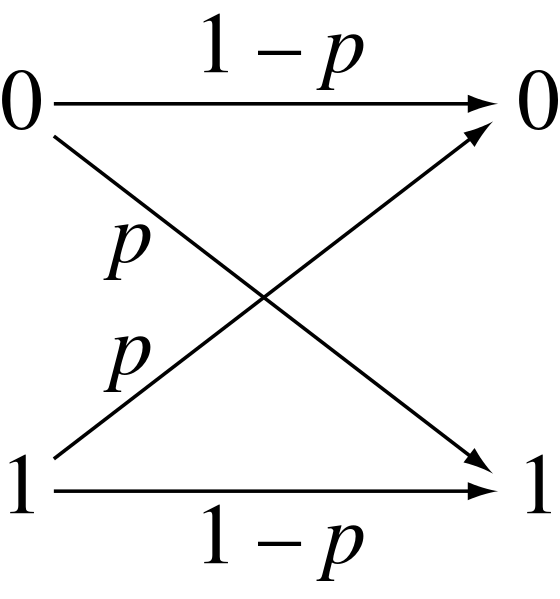
\includegraphics[scale=0.25]{Binary_symmetric_channel.png}

%\begin{tikzpicture}
%\draw[thick,->] (0,0) -- (6,-3) node[anchor=south east] {$\epsilon$}; 
%\draw[thick,->] (0,-3) -- (6,0) node[anchor=south east] {$\epsilon$}; 
%\end{tikzpicture}
\end{oss}
\section{Codici}
\label{sec:Codici}
In questo paragrafo daremo un idea di cioò che si intende con \textit{codice} in matematica per poi applicarci la nostra conoscenza sulla trasmissione di informazione.\\
\begin{defi}
L'\textbf{alfabeto di un codice, C} è un insieme \acode i cui elementi $c_i$ sono chiamati \textbf{simboli}.\\
Una \textbf{parola-codice} è una serie di simboli $c_{i_1}...c_{i_n}$. Il numero $n$ sarà la \textbf{lunghezza} della parola-codice.\\
Un \textbf{messaggio} sarà una successione di parole-codice.
\end{defi}
Il processo di codifica di un messaggio è quello di mappare ogni singolo  simbolo dell'alfabeto di un linguaggio con una parola-codice.\\
Un esempio di codice che poi utilizzeremo lungo tutto il capitolo è dato dal codice binario:
$$C=\{0, 1 \}$$
Il nostro obiettivo sarà ora capire cosa succede all'informazione trasmessa ora che il percorso sarà:
$$ SORGENTE \to codificatore \to CANALE \to decodificatore \to RICEVENTE$$
\\
Un'importantissima classe di codici è quella dei \textit{codici istantanei o codici prefisso}.
\begin{defi}
Sia $c_{i_1}...c_{i_n}$ una parola del codice. Preso $k<n$ se  $c_{i_1}...c_{i_k}$
è anch'essa una parola tale parola si dirà \textbf{prefisso}.\\
Un codice in cui non esistono parole che sono prefisso di altre è detto \textbf{codice istantaneo} o \textbf{codice prefisso}.
\end{defi}.
\begin{lem}
Ogni codice istantaneo è decodificabile in modo univoco, inoltre per avere una codifica univoca non è necessario aspettare di ricevere tutto il messaggio.
\end{lem}

Viste le sorprendenti proprietà dei codici istantanei è naturale chiederci quando è possibile creare codici con queste caratteristiche.

\begin{teo} \label{teo:disugKM} (\textit{Disugiaglianza di Kraft-McMillan})\\
Dato un alfabeto sorgente composto da $n$ simboli che deve essere codificato allora esiste un codice istantaneo con alfabeto di $r$ simboli e parole di lunghezza $l_i \ (1 \leq i \leq n)$ se e solo se 
\begin{equation}
\sumin r^{-l_i}\leq 1.
\end{equation} 
\end{teo}

Ora che, dato un alfabeto sorgente, abbiamo la possibilità di trovare dei codici che soddisfano le nostre richieste ci viene naturale domandarci come si può scegliere il migliore tra tutti i codici istantanei.

\begin{defi}
Dato un alfabeto sorgente $S$ \va con \lep a cui viene associato un codice istantaneo che traduce \va in $\{ l_1....\l_n \}$ posiamo considerare una variabile casuale $L$ con immagine $\{ l_1....\l_n \}$ e \lep , la stessa di $S$. Preso $\mathbb{E}(L)=\sumin p_j l_j$ il valore di aspettazione di $L$ diremo che \textbf{il codice è ottimale} se minimizza $\mathbb{E}(L)$.
\end{defi}
È chiaro che in generale un codice ottimale non è unico infatti dato un qualsiasi codice ottimale che utilizzi un alfabeto di almeno due lettere ci basterà considerare un codice in cui le lettere vengono permutate per ottenere un nuovo codice ottimale.
Enunciamo ora un sorprendente teorema che ci permette di mettere in relazione il codice ottimale con l'entropia dell'alfabeto sorgente.
 
\begin{teo}(\textit{Teorema della codifica di sorgente per simboli di codice})\\
Dato un alfabeto sorgente $S$ con \lep vale:
\begin{enumerate}
\item Per ogni codice istantaneo abbiamo che
\begin{equation}
\mathbb{E}(L)\geq \frac{H(S)}{\log (r)}
\end{equation}
con l'uguaglianza se e solo se $p_j=r^{l_j}$ $(1 \leq j \leq n)$
\item esiste un codice istantaneo per cui
\begin{equation}
\frac{H(S)}{\log (r)} \leq \mathbb{E}(L) < \frac{H(S)}{\log (r)} +1
\end{equation}
\end{enumerate}
\end{teo}

\begin{proof}
\item Definiamo $\{q_1...q_n \}$ con
\begin{equation}
q_j=\frac{r^{-l_j}}{\sumi r^{-l_i}}
\end{equation}
abbiamo scelto i $q_i$ in modo tale che 
$$\sumj q_j=1$$
e ovviamente $q_j\geq 0$.
Dunque $\{q_1...q_n \}$ è una distribuzione di probabilità e possiamo quindi utilizzare la Disuguaglianza di Gibbs nel caso discreto: $- \sumin p_i \log(p_i) \leq -sumin p_i \log(q_i)$ con $\{p_1...p_n \}$ e $\{q_1...q_n \}$ distribuzioni di probabilità (deriva quasi immediatamente da \ref{teo:GibbsContinuo}).\\
\[
\begin{split}
H(S)& = - \sumj p_j \log(p_j) \\
& \leq  - \sumj p_j \log(q_j)\\
& =  - \sumj p_j \log \bigg(\frac{r^{-l_j}}{\sumi r^{-l_i}} \bigg)\\
& =  - \sumj p_j \log ( r^{-l_j}) +\sumj p_j \log \bigg( \sumi r^{-l_i} \bigg)\\
& \leq - \sumj p_j \log ( r^{-l_j}) +\sumj p_j \log (1)\\
& =\sumj p_j l_j \log ( r)\\
&= \mathbb{E}(L)\log (r)
\end{split}
\]
dove per ottenere la quinta riga abbiamo utilizzato la disugiaglianza di Kraft-McMillan \ref{teo:disugKM}.\\
Dalle condizioni delle disuguaglianze di Gibbs e Kraft abbiamo che si ha l'uguaglianza se e solo se $p_j=r^{-l_j}$
\item  Il primo punto dimostra anche il primo membro della disuguaglianza, mostriamo ora la validità della seconda parte.\\
Imponiamo $l_j =  -\lceil \log_r(p_j) \rceil$ cioè  $- \log_r(p_j) \leq l_j < - \log_r(p_j) +1$ e quindi 
$$r^{-l_j} \leq p_j \implies $$ 
$$  \sumj r^{-l_j} \leq \sumj p_j=1.$$
Quindi per la disuguaglianza di Kraft esiste un codice di tale lunghezza con variabile casuale associata $L$. Abbiamo:
 \[
\begin{split}
H(L)& =  \sumj p_j l_j \\
& <   - \sumj p_j  \log_r(p_j) +1\\
& = - \sumj p_j  \frac{\log(p_j)}{\log(r)} +1 \\
& =  \frac{H(S)}{ \log (r)} +1
\end{split}
\]
\end{proof}
Il teorema appena dimostrato è detto primo teorema di Shannon e fu dimostrato proprio dal matematico Americano nel 1948.\\


\section{Regole di decisione}
Mettiamoci nella situazione
$$ SORGENTE \to codificatore \to CANALE \to decodificatore \to RICEVENTE$$
e concentriamoci sul segmento $codificatore \to CANALE \to decodificatore$.\\
Supponiamo che $C:=\{ x_1 ..x_n \}$ sia l'insieme di tutte le possibili parole del codice che possono essere trasmesse dal e che $y$ sia la parola ricevuta. Per decidere quale parola $x_i$ è stata trasmessa possiamo utilizzare il \textit{principio di massima verosimiglianza}:\\
Date le probabilità condizionate $p(y|x_i):=(R=y|X=x_i)$ decideremo che la parola inviata è $x_k$ se
\begin{equation} \label{eq6}
p(y|x_k )\geq p(y=x_i) \ \forall i
\end{equation}
Nel caso in cui più $x_s$ soddisfino \ref{eq6} $x_k$ verrà scelta in modo casuale tra le varie $x_s$.\\
Ovviamente la nostra scelta di $x_k$ non ci garantisce che sia stata effettivamente inviata $x_k$.\\
Esistono altri principi sui quali basarsi per la scelta di $x_k$ nel caso di codici binari ad esempio si può definire \textit{distanza di Hammning} per aiutarsi nella decisione:
\begin{defi}
date due parole di un codice binario $a,b$ si definisce \textbf{distanza di Hamming} il numero di simboli per cui $a$ è differente da $b$
\end{defi}
Utilizzando questa distanza è naturale scegliere come parola $x_k$ inviata quella che dista meno dalla parola ricevuta $y$.

\begin{teo}
Per un canale binario simmetrico come quello visto in \textbf{Osservazione} \ref{oss:bsc} dove $0 \leq p < \frac{1}{2}$, fissata una parola $y$ l'insieme $\{ x_s \}$ delle parole con distanza di Hamming minima da $y$ coincide con quello delle parole a verosimiglianza massima rispetto a $y$
\end{teo}
\begin{proof}
Sia $m$ la lunghezza di $y$, la probabilità che sia stata inviata una parola $x$ tale che $d(x,y)=\epsilon \leq m$ è:
$$\mathbb{P}(Y=y|X=x)= p^{\epsilon}(1-p)^{m-\epsilon}=(1-p)^m \bigg( \frac{p}{1-p} \bigg)^{\epsilon}$$
Dato che $0 \leq p < \frac{1}{2} \implies \frac{p}{1-p}<1 $ e quindi $\mathbb{P}(Y=y|X=x)$ ha massimo quando $\epsilon$ è minimo.
\end{proof}







